\chapter{Approche algorithmique séquentielle}

\epigraph{\textit{``The art of programming is the art of organizing complexity.''}}{--- Edsger W. Dijkstra}

\section{Backtracking et Branch-and-Bound : principe général}

\subsection{Le backtracking}

Le \textbf{backtracking} (retour sur trace) est une technique algorithmique de recherche exhaustive qui explore systématiquement l'espace des solutions possibles en construisant incrémentalement des solutions partielles. Lorsqu'une solution partielle ne peut plus mener à une solution valide, l'algorithme \textit{revient en arrière} pour explorer d'autres branches.

\begin{definition}[Backtracking]
Le backtracking construit un arbre de recherche où :
\begin{itemize}
    \item Chaque \textbf{nœud} représente une solution partielle (un préfixe de règle de Golomb) ;
    \item Chaque \textbf{arête} représente l'ajout d'une nouvelle marque ;
    \item Les \textbf{feuilles} sont soit des solutions complètes, soit des impasses.
\end{itemize}
\end{definition}

Pour le problème OGR, une solution partielle est un ensemble de marques $\{0, m_1, \ldots, m_k\}$ avec $k < n$ qui satisfait déjà la propriété de Golomb (toutes les différences distinctes).

\begin{figure}[H]
\centering
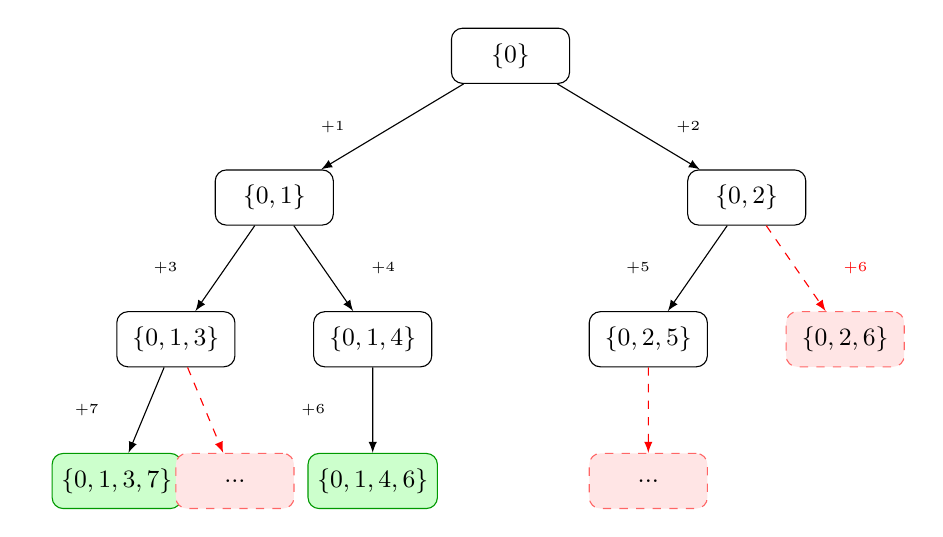
\begin{tikzpicture}[
    level distance=1.8cm,
    sibling distance=3cm,
    edge from parent/.style={draw, -latex},
    every node/.style={draw, rounded corners, minimum width=1.5cm, minimum height=0.7cm, align=center, font=\small},
    level 1/.style={sibling distance=6cm},
    level 2/.style={sibling distance=2.5cm},
    level 3/.style={sibling distance=1.5cm},
    pruned/.style={draw=red!60, fill=red!10, dashed},
    solution/.style={draw=green!60!black, fill=green!20},
]
    \node {$\{0\}$}
        child { node {$\{0,1\}$}
            child { node {$\{0,1,3\}$}
                child { node[solution] {$\{0,1,3,7\}$} edge from parent node[left, draw=none, font=\tiny] {+7} }
                child { node[pruned] {...} edge from parent[dashed, red] }
                edge from parent node[left, draw=none, font=\tiny] {+3}
            }
            child { node {$\{0,1,4\}$}
                child { node[solution] {$\{0,1,4,6\}$} edge from parent node[left, draw=none, font=\tiny] {+6} }
                edge from parent node[right, draw=none, font=\tiny] {+4}
            }
            edge from parent node[left, draw=none, font=\tiny] {+1}
        }
        child { node {$\{0,2\}$}
            child { node {$\{0,2,5\}$}
                child { node[pruned] {...} edge from parent[dashed, red] }
                edge from parent node[left, draw=none, font=\tiny] {+5}
            }
            child { node[pruned] {$\{0,2,6\}$} edge from parent[dashed, red] node[right, draw=none, font=\tiny] {+6} }
            edge from parent node[right, draw=none, font=\tiny] {+2}
        };
\end{tikzpicture}
\caption{Arbre de recherche par backtracking pour $n=4$. Les nœuds rouges sont élagués, les verts sont des solutions.}
\label{fig:backtrack_tree}
\end{figure}

\subsection{Le Branch-and-Bound}

Le \textbf{branch-and-bound} (séparation et évaluation) enrichit le backtracking en ajoutant des \textbf{bornes} permettant d'élaguer (pruning) les branches qui ne peuvent pas mener à une solution meilleure que la meilleure solution connue.

\begin{important}{Principe du Branch-and-Bound}
À chaque nœud de l'arbre de recherche :
\begin{enumerate}
    \item Calculer une \textbf{borne inférieure} $LB$ de la meilleure solution atteignable depuis ce nœud ;
    \item Si $LB \geq$ meilleure solution connue, \textbf{élaguer} cette branche ;
    \item Sinon, \textbf{explorer} les sous-branches (branching).
\end{enumerate}
\end{important}

L'efficacité du branch-and-bound dépend de deux facteurs :
\begin{itemize}
    \item La \textbf{qualité des bornes} : plus elles sont serrées, plus l'élagage est efficace ;
    \item L'\textbf{ordre d'exploration} : trouver rapidement de bonnes solutions améliore les bornes.
\end{itemize}

\subsection{Application au problème OGR}

Pour la recherche de règles de Golomb optimales, l'algorithme procède ainsi :

\begin{enumerate}
    \item Initialiser avec les marques $\{0\}$ et une borne supérieure $bestLen$ (longueur maximale acceptable) ;
    \item Pour chaque position candidate $next > m_{k-1}$ :
    \begin{enumerate}
        \item Vérifier que $next$ ne crée pas de conflit (différence déjà utilisée) ;
        \item Vérifier que la borne inférieure ne dépasse pas $bestLen$ ;
        \item Si valide : ajouter $next$ aux marques et continuer récursivement ;
    \end{enumerate}
    \item Si $k = n$ : on a une solution complète, mettre à jour $bestLen$ si meilleure ;
    \item Sinon : backtrack (retirer $next$ et essayer la position suivante).
\end{enumerate}

\section{Stratégies de pruning}

L'efficacité de la recherche repose sur l'identification rapide des branches non prometteuses. Plusieurs stratégies de pruning sont implémentées.

\subsection{Coupe sur la borne supérieure}

La coupe la plus simple : si la position candidate $next$ atteint ou dépasse la meilleure longueur connue, elle est rejetée.

\begin{algorithm}[H]
\caption{Coupe sur la borne supérieure}
\begin{algorithmic}[1]
\State $upperBound \gets bestLen - 1$ \Comment{On veut strictement mieux}
\For{$next \gets lastMark + 1$ \textbf{to} $upperBound$}
    \State \Comment{Explorer seulement si $next < bestLen$}
\EndFor
\end{algorithmic}
\end{algorithm}

Cette coupe est triviale mais essentielle : elle garantit que toute solution trouvée améliore strictement la meilleure connue.

\subsection{Borne inférieure de Golomb}

Une borne plus sophistiquée utilise le nombre de marques restantes à placer :

\begin{theorem}[Borne inférieure dynamique]
Soit une solution partielle avec $k$ marques et dernière marque à la position $L_k$. S'il reste $r = n - k$ marques à placer, alors la longueur finale minimale est :
\begin{equation}
L_{min} = L_k + \frac{r(r+1)}{2}
\end{equation}
\end{theorem}

\begin{proof}
Les $r$ marques restantes créeront au moins $r$ nouvelles différences (entre chaque nouvelle marque et la dernière). Ces différences minimales sont $1, 2, \ldots, r$, donc l'extension minimale est $1 + 2 + \cdots + r = \frac{r(r+1)}{2}$.
\end{proof}

\begin{figure}[H]
\centering
\begin{tikzpicture}[scale=0.6]
    % Règle actuelle
    \draw[thick] (0,0) -- (16,0);
    \foreach \x in {0,2,4,6,8,10,12,14,16} {
        \draw (\x,-0.1) -- (\x,0.1);
    }

    % Marques existantes
    \foreach \x in {0,2,8} {
        \draw[fill=burgundy, burgundy, thick] (\x,-0.3) -- (\x,0.6);
        \draw[fill=burgundy] (\x,0.6) circle (0.12);
    }

    % Extension minimale
    \draw[<->, gold, thick] (8,-0.8) -- (9,-0.8) node[midway, below] {\small +1};
    \draw[<->, gold, thick] (9,-1.4) -- (11,-1.4) node[midway, below] {\small +2};
    \draw[<->, gold, thick] (11,-0.8) -- (14,-0.8) node[midway, below] {\small +3};

    % Marques futures (pointillées)
    \foreach \x in {9,11,14} {
        \draw[fill=gold!50, gold, thick, dashed] (\x,-0.3) -- (\x,0.6);
        \draw[fill=gold!50, dashed] (\x,0.6) circle (0.12);
    }

    % Annotations
    \node[above] at (0, 0.8) {$0$};
    \node[above] at (2, 0.8) {$m_1$};
    \node[above] at (8, 0.8) {$L_k$};
    \node[above, gold] at (14, 0.8) {$L_{min}$};

    % Formule
    \node[align=center] at (8, -3) {$r = 3$ marques restantes $\Rightarrow$ extension minimale = $\frac{3 \times 4}{2} = 6$};
\end{tikzpicture}
\caption{Illustration de la borne inférieure dynamique avec $r=3$ marques restantes}
\label{fig:lower_bound}
\end{figure}

L'implémentation dans notre code :

\begin{lstlisting}[language=C++, caption={Pruning par borne inférieure}]
const int r = n - numMarks;  // marques restantes
const int minAdditionalLength = (r * (r + 1)) / 2;

if (lastMark + minAdditionalLength >= state.bestLen) {
    // Elaguer: impossible d'améliorer bestLen
    continue;
}
\end{lstlisting}

\subsection{Borne supérieure dynamique}

On peut également borner la position maximale pour la prochaine marque :

\begin{equation}
next_{max} = bestLen - 1 - \frac{(r-1) \cdot r}{2}
\end{equation}

Cette borne anticipe que les $(r-1)$ marques après $next$ devront au minimum ajouter $\frac{(r-1)r}{2}$ à la longueur.

\begin{lstlisting}[language=C++, caption={Calcul de la borne supérieure pour next}]
const int max_remaining = ((r - 1) * r) / 2;
const int max_pos = state.bestLen - max_remaining - 1;

for (int pos = min_pos; pos <= max_pos; ++pos) {
    // Explorer uniquement les positions viables
}
\end{lstlisting}

\subsection{Comparaison des stratégies}

\begin{table}[H]
\centering
\begin{tabular}{lcc}
\toprule
\textbf{Stratégie} & \textbf{Complexité calcul} & \textbf{Efficacité élagage} \\
\midrule
$next < bestLen$ & $O(1)$ & Faible \\
Borne inférieure Golomb & $O(1)$ & Moyenne à forte \\
Borne supérieure dynamique & $O(1)$ & Moyenne \\
Combinaison & $O(1)$ & Forte \\
\bottomrule
\end{tabular}
\caption{Comparaison des stratégies de pruning}
\label{tab:pruning_strategies}
\end{table}

\section{Réduction de symétrie}

\subsection{Principe de la symétrie}

Comme vu au chapitre précédent, chaque règle de Golomb possède une \textbf{règle miroir} équivalente obtenue par réflexion. Explorer les deux est redondant et double le temps de calcul.

\begin{example}
$\{0, 1, 4, 6\}$ et $\{0, 2, 5, 6\}$ sont miroirs :
\begin{align*}
\{0, 1, 4, 6\} &\xrightarrow{\text{miroir}} \{6-6, 6-4, 6-1, 6-0\} = \{0, 2, 5, 6\}
\end{align*}
\end{example}

\subsection{Stratégie de réduction}

Pour éviter d'explorer les paires de règles miroirs, nous imposons des contraintes qui sélectionnent une seule forme canonique.

\subsubsection{Contrainte sur la première marque}

\begin{theorem}[Symmetry Breaking 1]
Pour toute règle de Golomb $\{0, m_1, \ldots, m_{n-1}\}$ et son miroir, au moins une satisfait :
\begin{equation}
m_1 \leq \frac{L}{2}
\end{equation}
où $L = m_{n-1}$ est la longueur de la règle.
\end{theorem}

En pratique, on restreint la boucle sur $m_1$ (appelée \texttt{firstMark}) :

\begin{lstlisting}[language=C++, caption={Symmetry breaking sur la première marque}]
// SYMMETRY BREAKING: a_1 <= bestLen/2
for (int firstMark = 1; firstMark <= state.bestLen / 2; ++firstMark) {
    // Explorer seulement la moitie gauche
}
\end{lstlisting}

Cette contrainte élimine environ \textbf{50\%} des branches explorées.

\subsubsection{Contrainte sur la dernière marque}

Une contrainte plus fine vérifie au moment de compléter une solution :

\begin{theorem}[Symmetry Breaking 2]
Une règle $\{0, m_1, \ldots, m_{n-1}\}$ est en forme canonique si :
\begin{equation}
m_1 < m_{n-1} - m_{n-2}
\end{equation}
\end{theorem}

Cette condition compare le premier écart ($m_1 - 0 = m_1$) au dernier écart ($m_{n-1} - m_{n-2}$). La règle canonique est celle dont le premier écart est plus petit.

\begin{lstlisting}[language=C++, caption={Symmetry breaking à la solution}]
if (newNumMarks == n) {
    // Symmetry breaking: m_1 < m_{n-1} - m_{n-2}
    // Equivalent: next > lastMark + marks[1]
    if (next <= lastMark + marks[1]) {
        continue;  // Skip le miroir
    }
    // Accepter cette solution
}
\end{lstlisting}

\subsection{Impact attendu}

La réduction de symétrie divise théoriquement l'espace de recherche par 2. En pratique, le gain dépend de la distribution des solutions :

\begin{itemize}
    \item \textbf{Gain maximal} : si les solutions sont uniformément distribuées, speedup $\approx 2\times$ ;
    \item \textbf{Gain réel} : souvent entre $1.5\times$ et $2\times$ car certaines branches miroirs sont déjà élaguées par d'autres prunings.
\end{itemize}

\begin{figure}[H]
\centering
\begin{tikzpicture}[scale=0.8]
    % Sans symétrie
    \draw[fill=burgundy!30] (0,0) rectangle (3,4);
    \node at (1.5, 4.3) {Sans réduction};
    \node at (1.5, 2) {100\%};

    % Avec symétrie
    \draw[fill=gold!30] (5,0) rectangle (8,2);
    \draw[fill=gray!20, pattern=north east lines] (5,2) rectangle (8,4);
    \node at (6.5, 4.3) {Avec réduction};
    \node at (6.5, 1) {$\sim$50\%};
    \node[gray] at (6.5, 3) {éliminé};

    % Légende
    \draw[fill=gold!30] (10,3.5) rectangle (10.5,4);
    \node[right] at (10.6, 3.75) {Exploré};
    \draw[fill=gray!20, pattern=north east lines] (10,2.5) rectangle (10.5,3);
    \node[right] at (10.6, 2.75) {Éliminé (miroir)};
\end{tikzpicture}
\caption{Impact de la réduction de symétrie sur l'espace de recherche}
\label{fig:symmetry_impact}
\end{figure}

\section{Représentation binaire des distances}

\subsection{Motivation}

La vérification des collisions (une nouvelle différence existe-t-elle déjà ?) est l'opération la plus fréquente. L'utilisation d'un \textbf{bitset} permet des opérations en temps constant.

\subsection{Structure \texttt{bitset} classique}

Un bitset de taille $M$ (où $M$ est la longueur maximale) représente les différences utilisées :
\begin{itemize}
    \item Le bit $d$ est à 1 si la différence $d$ est déjà utilisée ;
    \item Test de collision : $O(1)$ avec \texttt{seen[d]} ;
    \item Ajout d'une différence : $O(1)$ avec \texttt{seen.set(d)}.
\end{itemize}

\begin{lstlisting}[language=C++, caption={Opérations sur bitset standard}]
std::bitset<MAX_DIFF> usedDiffs;

// Test de collision
if (usedDiffs[d]) {
    // Collision! Cette difference existe deja
}

// Marquer une difference
usedDiffs.set(d);
\end{lstlisting}

\subsection{Structure \texttt{BitSet128} optimisée}

Pour maximiser les performances, nous utilisons une structure personnalisée basée sur deux \texttt{uint64\_t} :

\begin{lstlisting}[language=C++, caption={Structure BitSet128}]
struct alignas(16) BitSet128 {
    uint64_t lo;  // bits 0-63
    uint64_t hi;  // bits 64-127

    // Set bit at position
    inline void set(int pos) {
        if (pos < 64) lo |= (1ULL << pos);
        else          hi |= (1ULL << (pos - 64));
    }

    // Test bit at position
    inline bool test(int pos) const {
        if (pos < 64) return (lo >> pos) & 1;
        else          return (hi >> (pos - 64)) & 1;
    }

    // Check if any bit is set
    inline bool any() const {
        return (lo | hi) != 0;
    }
};
\end{lstlisting}

\subsection{Optimisation clé : détection de collision en O(1)}

L'innovation majeure de la version V2 est l'utilisation du \textbf{décalage de bits} pour calculer toutes les nouvelles différences en une seule opération.

\subsubsection{Encodage des marques inversées}

Au lieu de stocker les positions des marques, on encode leur position \textit{relative à la longueur courante} :

\begin{defi}{Reversed Marks}
Pour une règle partielle $\{0, m_1, \ldots, m_k\}$ de longueur $L_k = m_k$, le bitset \texttt{reversed\_marks} a le bit $i$ à 1 si et seulement si il existe une marque à la position $L_k - i$.
\end{defi}

\begin{example}
Pour $\{0, 1, 4, 9\}$ avec $L_k = 9$ :
\begin{itemize}
    \item Marque 0 $\rightarrow$ bit à position $9 - 0 = 9$
    \item Marque 1 $\rightarrow$ bit à position $9 - 1 = 8$
    \item Marque 4 $\rightarrow$ bit à position $9 - 4 = 5$
    \item Marque 9 $\rightarrow$ bit à position $9 - 9 = 0$
\end{itemize}
\texttt{reversed\_marks} = bits aux positions $\{0, 5, 8, 9\}$
\end{example}

\subsubsection{Calcul des différences par shift}

Lorsqu'on ajoute une marque à la position $pos$, le décalage $offset = pos - L_k$ permet de calculer toutes les nouvelles différences :

\begin{equation}
\texttt{new\_dist} = \texttt{reversed\_marks} \ll offset
\end{equation}

\begin{theorem}[Correction du shift]
Si le bit $i$ est à 1 dans \texttt{reversed\_marks} (marque à $L_k - i$), alors le bit $i + offset$ sera à 1 dans \texttt{new\_dist}. Or $i + offset = i + (pos - L_k) = pos - (L_k - i)$, qui est exactement la différence entre la nouvelle marque et l'ancienne.
\end{theorem}

\begin{figure}[H]
\centering
\begin{tikzpicture}[scale=0.5]
    % reversed_marks avant shift
    \node[anchor=east] at (-1, 3) {\small reversed\_marks :};
    \draw (0,2.5) rectangle (16,3.5);
    \foreach \x in {0,1,...,15} {
        \draw (\x,2.5) -- (\x,3.5);
        \node[above, font=\tiny] at (\x+0.5, 3.5) {\x};
    }
    % Bits actifs: positions 0, 5, 8, 9
    \foreach \x in {0,5,8,9} {
        \fill[burgundy] (\x+0.1,2.6) rectangle (\x+0.9,3.4);
    }

    % Flèche
    \draw[->, thick] (8, 2) -- (8, 1) node[midway, right] {\small $\ll 3$};

    % new_dist après shift
    \node[anchor=east] at (-1, 0) {\small new\_dist :};
    \draw (0,-0.5) rectangle (16,0.5);
    \foreach \x in {0,1,...,15} {
        \draw (\x,-0.5) -- (\x,0.5);
    }
    % Bits décalés: positions 3, 8, 11, 12
    \foreach \x in {3,8,11,12} {
        \fill[gold] (\x+0.1,-0.4) rectangle (\x+0.9,0.4);
    }

    % Explication
    \node[align=left, anchor=west] at (17, 1.5) {\small Nouvelles différences :\\  \small $\{3, 8, 11, 12\}$};
\end{tikzpicture}
\caption{Calcul des différences par décalage : ajout d'une marque avec $offset = 3$}
\label{fig:shift_operation}
\end{figure}

\subsubsection{Test de collision}

Une fois \texttt{new\_dist} calculé, le test de collision est un simple AND :

\begin{lstlisting}[language=C++, caption={Test de collision O(1)}]
BitSet128 new_dist = reversed_marks << offset;

// Collision si une difference existe deja
if ((new_dist & used_dist).any()) {
    continue;  // Rejeter ce candidat
}
\end{lstlisting}

\subsection{Invariants maintenus}

À tout instant de la recherche, les invariants suivants sont maintenus :

\begin{enumerate}
    \item \texttt{used\_dist} contient exactement les $\binom{k}{2}$ différences des $k$ marques placées ;
    \item \texttt{reversed\_marks} encode les $k$ marques relativement à la longueur courante ;
    \item Aucune collision n'existe : \texttt{(reversed\_marks \& used\_dist) == 0}.
\end{enumerate}

\section{Pseudo-code de la recherche}

\subsection{Version récursive conceptuelle}

L'algorithme peut être exprimé récursivement de façon claire :

\begin{algorithm}[H]
\caption{Recherche OGR par backtracking récursif}
\label{alg:recursive}
\begin{algorithmic}[1]
\Procedure{Search}{$marks$, $usedDist$, $n$, $bestLen$}
    \State $k \gets |marks|$
    \State $lastMark \gets marks[k-1]$

    \Statex
    \State \Comment{=== PRUNING: Borne inférieure ===}
    \State $r \gets n - k$ \Comment{Marques restantes}
    \If{$lastMark + \frac{r(r+1)}{2} \geq bestLen$}
        \State \Return \Comment{Élaguer cette branche}
    \EndIf

    \Statex
    \State \Comment{=== EXPLORATION ===}
    \For{$next \gets lastMark + 1$ \textbf{to} $bestLen - 1$}

        \Statex
        \State \Comment{Test de validité (différences)}
        \State $valid \gets \textsc{True}$
        \For{$i \gets 0$ \textbf{to} $k-1$}
            \State $d \gets next - marks[i]$
            \If{$d \in usedDist$}
                \State $valid \gets \textsc{False}$
                \State \textbf{break}
            \EndIf
        \EndFor

        \Statex
        \If{$\neg valid$}
            \State \textbf{continue}
        \EndIf

        \Statex
        \State \Comment{=== CANDIDAT VALIDE ===}
        \If{$k + 1 = n$}
            \State \Comment{Solution complète trouvée}
            \If{$next < bestLen$ \textbf{and} \textsc{IsCanonical}($marks$, $next$)}
                \State $bestLen \gets next$
                \State \textsc{SaveSolution}($marks$, $next$)
            \EndIf
        \Else
            \State \Comment{Récursion}
            \State $newDists \gets \{next - marks[i] : i \in [0, k-1]\}$
            \State \textsc{Search}($marks \cup \{next\}$, $usedDist \cup newDists$, $n$, $bestLen$)
        \EndIf
    \EndFor
\EndProcedure
\end{algorithmic}
\end{algorithm}

\subsection{Version itérative avec pile}

Pour éviter l'overhead des appels de fonction, notre implémentation utilise une \textbf{pile manuelle} :

\begin{algorithm}[H]
\caption{Recherche OGR itérative avec pile}
\label{alg:iterative}
\begin{algorithmic}[1]
\Procedure{SearchIterative}{$n$, $maxLen$}
    \State $stack \gets$ pile pré-allouée de $n$ frames
    \State $bestLen \gets maxLen + 1$

    \Statex
    \State \Comment{=== SYMMETRY BREAKING: $m_1 \leq bestLen/2$ ===}
    \For{$firstMark \gets 1$ \textbf{to} $bestLen / 2$}
        \State Initialiser $stack[0]$ avec $\{0, firstMark\}$
        \State $stackTop \gets 0$

        \Statex
        \While{$stackTop \geq 0$}
            \State $frame \gets stack[stackTop]$

            \Statex
            \State \Comment{Pruning}
            \If{borne inférieure $\geq bestLen$}
                \State $stackTop \gets stackTop - 1$
                \State \textbf{continue}
            \EndIf

            \Statex
            \State \Comment{Exploration des candidats}
            \State $pushed \gets \textsc{False}$
            \For{$next \gets frame.nextCandidate$ \textbf{to} $upperBound$}
                \If{\textsc{HasCollision}($frame$, $next$)}
                    \State \textbf{continue}
                \EndIf

                \Statex
                \If{$frame.numMarks + 1 = n$}
                    \State Mettre à jour $bestLen$ si amélioration
                \Else
                    \State $frame.nextCandidate \gets next + 1$
                    \State Push nouveau frame vers $stack[stackTop + 1]$
                    \State $stackTop \gets stackTop + 1$
                    \State $pushed \gets \textsc{True}$
                    \State \textbf{break}
                \EndIf
            \EndFor

            \Statex
            \If{$\neg pushed$}
                \State $stackTop \gets stackTop - 1$ \Comment{Backtrack}
            \EndIf
        \EndWhile
    \EndFor

    \State \Return meilleure solution
\EndProcedure
\end{algorithmic}
\end{algorithm}

\subsection{Placement des tests}

Le schéma suivant résume où interviennent les différents tests dans la boucle principale :

\begin{figure}[H]
\centering
\begin{tikzpicture}[
    node distance=0.8cm,
    startstop/.style={rectangle, rounded corners, draw=burgundy, fill=burgundy!20, text width=4cm, align=center, minimum height=0.8cm},
    process/.style={rectangle, draw=gold!80!black, fill=gold!20, text width=5cm, align=center, minimum height=0.8cm},
    decision/.style={diamond, draw=burgundy, fill=burgundy!10, text width=2.5cm, align=center, aspect=2},
    arrow/.style={thick,->,>=stealth}
]
    \node[startstop] (start) {Début frame};
    \node[decision, below=of start] (bound) {Borne inf. $\geq$ bestLen ?};
    \node[startstop, right=2cm of bound] (prune1) {Élaguer (pop)};
    \node[process, below=of bound] (loop) {Pour chaque $next$};
    \node[decision, below=of loop] (collision) {Collision ?};
    \node[startstop, right=2cm of collision] (skip) {Skip (continue)};
    \node[decision, below=of collision] (complete) {Solution complète ?};
    \node[process, right=2cm of complete] (update) {Maj bestLen};
    \node[process, below=of complete] (push) {Push nouveau frame};

    \draw[arrow] (start) -- (bound);
    \draw[arrow] (bound) -- node[above] {oui} (prune1);
    \draw[arrow] (bound) -- node[right] {non} (loop);
    \draw[arrow] (loop) -- (collision);
    \draw[arrow] (collision) -- node[above] {oui} (skip);
    \draw[arrow] (collision) -- node[right] {non} (complete);
    \draw[arrow] (complete) -- node[above] {oui} (update);
    \draw[arrow] (complete) -- node[right] {non} (push);

    % Retours
    \draw[arrow, dashed] (skip) |- (loop);
    \draw[arrow, dashed] (update) |- (loop);
\end{tikzpicture}
\caption{Flux de contrôle et placement des tests dans la boucle de recherche}
\label{fig:control_flow}
\end{figure}

\subsection{Complexité}

\begin{itemize}
    \item \textbf{Pire cas} : $O(L^n)$ où $L$ est la longueur maximale (exploration exhaustive) ;
    \item \textbf{Cas moyen} : drastiquement réduit par le pruning, mais reste exponentiel ;
    \item \textbf{Espace} : $O(n)$ pour la pile (profondeur maximale = $n$ niveaux).
\end{itemize}

Les optimisations (bitset, pruning, symétrie) ne changent pas la complexité asymptotique mais réduisent considérablement les constantes, permettant de traiter des instances plus grandes en temps raisonnable.
